% !TEX program = xelatex
\PassOptionsToPackage{unicode=true}{hyperref} % options for packages loaded elsewhere
\PassOptionsToPackage{hyphens}{url}

%
\documentclass[]{article}
\usepackage{lmodern}
\usepackage{amssymb,amsmath}
\usepackage{ifxetex,ifluatex}
\usepackage{fixltx2e} % provides \textsubscript
\ifnum 0\ifxetex 1\fi\ifluatex 1\fi=0 % if pdftex
  \usepackage[T1]{fontenc}
  \usepackage[utf8]{inputenc}
  \usepackage{textcomp} % provides euro and other symbols
\else % if luatex or xelatex
  \usepackage{unicode-math}
  \defaultfontfeatures{Ligatures=TeX,Scale=MatchLowercase}
\fi
% use upquote if available, for straight quotes in verbatim environments
\IfFileExists{upquote.sty}{\usepackage{upquote}}{}
% use microtype if available
\IfFileExists{microtype.sty}{%
    \usepackage[]{microtype}
    \UseMicrotypeSet[protrusion]{basicmath} % disable protrusion for tt fonts
}{}
\IfFileExists{parskip.sty}{%
\usepackage{parskip}
    }{% else
    \setlength{\parindent}{0pt}
    \setlength{\parskip}{6pt plus 2pt minus 1pt}
}
\usepackage{hyperref}
% \hypersetup{
%             pdfborder={0 0 0},
%             breaklinks=true}
\urlstyle{same}  % don't use monospace font for urls
\usepackage{graphicx,grffile}
\makeatletter
\def\maxwidth{\ifdim\Gin@nat@width>\linewidth\linewidth\else\Gin@nat@width\fi}
\def\maxheight{\ifdim\Gin@nat@height>\textheight\textheight\else\Gin@nat@height\fi}
\makeatother
% Scale images if necessary, so that they will not overflow the page
% margins by default, and it is still possible to overwrite the defaults
% using explicit options in \includegraphics[width, height, ...]{}
\setkeys{Gin}{width=\maxwidth,height=\maxheight,keepaspectratio}
\usepackage[normalem]{ulem}
% avoid problems with \sout in headers with hyperref:
\pdfstringdefDisableCommands{\renewcommand{\sout}{}}
\setlength{\emergencystretch}{3em}  % prevent overfull lines
\providecommand{\tightlist}{%
  \setlength{\itemsep}{0pt}\setlength{\parskip}{0pt}}
% \setcounter{secnumdepth}{0}
% Redefines (sub)paragraphs to behave more like sections
\ifx\paragraph\undefined\else
\let\oldparagraph\paragraph
\renewcommand{\paragraph}[1]{\oldparagraph{#1}\mbox{}}
\fi
\ifx\subparagraph\undefined\else
\let\oldsubparagraph\subparagraph
\renewcommand{\subparagraph}[1]{\oldsubparagraph{#1}\mbox{}}
\fi

% set default figure placement to htbp
\makeatletter
\def\fps@figure{htbp}
\makeatother
\title{
    Summary for Jingtun ZHANG's 2019 Summer Intern \\
    @\href{https://ucsb.edu}{University of California Santa Barbara}
}
\author{
    Jingtun ZHANG 张劲暾
}
\date{  16th September, 2019   }


\usepackage{geometry}
\usepackage[colorlinks,urlcolor=blue,dvipdfm]{hyperref}

\geometry{left=1.5cm,right=1.5cm,top=2cm,bottom=2cm}

\begin{document}
\maketitle
% \newpage
\tableofcontents
% \newpage
\hypertarget{header-n1761}{%
\section{Introduction}\label{header-n1761}}

This is a summary of Jingtun ZHANG's 2019 summer intern
@\href{https://ucsb.edu}{University of California Santa Barbara}

\begin{quote}
Paper reading note can be found at
\href{https://github.com/OrdinaryCrazy/cnn-compiler-notebook/tree/master/paper-reading-note}{Github
link}

Studying note can be found at
\href{https://github.com/OrdinaryCrazy/cnn-compiler-notebook/tree/master/Studying\%20Note}{Github
link}

Weekly report can be found at
\href{https://github.com/OrdinaryCrazy/cnn-compiler-notebook/tree/master/weekly-report}{Github
link}
\end{quote}




\hypertarget{header-n1768}{%
\section{Graph Neural Network Survey}\label{header-n1768}}

\hypertarget{header-n1769}{%
\subsection{Background}\label{header-n1769}}

\hypertarget{header-n1770}{%
\subsubsection{Origin GNN}\label{header-n1770}}

\textbf{Target problem}: learn a state embedding
\(\mathbf{h}_v\in \mathbb{R}^{s}\) for each node

\textbf{Traditional procedure}:

\(\mathbf{h}_{v} = f(\mathbf{x}_v,edge\_attr_v,\mathbf{h}_u,\mathbf{x}_u)\)\\
\(u\) means neighbors of \(v\), \(f\) is local parameterized transition
function\\
\(\mathbf{o}_v = g(\mathbf{h}_v, \mathbf{x}_v)\)\\
\(g\) is local output function

\textbf{Typical loss}:

\(loss = \sum_{i = 1}^{p}(target_i - output_i)\)

Details can be found at
\href{https://github.com/OrdinaryCrazy/cnn-compiler-notebook/blob/master/Studying\%20Note/README.md}{Github
link}

\hypertarget{header-n1777}{%
\subsubsection{From spectral to propagation: Graph Convolutional Network
(GCN)}\label{header-n1777}}

\textbf{\(g_\theta(\Lambda)\) can be well-approximated by a truncated
expansion in terms of Chebyshev polynomials \(T_k(x)\) up to \(K^{th}\)
order:}

\(g_{\theta'}(\Lambda) \approx \sum^{K}_{k=0}\theta^{'}_{k} T_k(\widetilde{\Lambda})\)

\begin{enumerate}
\def\labelenumi{\arabic{enumi}.}
\item
  \(\widetilde{\Lambda} = \frac{2}{\lambda_{max}} \Lambda - I_N\),
  \(\lambda_{max}\) denotes the largest eigenvalue of \(L\)
\item
  \(\theta' \in \mathbb{R}^{K}\): vector of Chebyshev coefficients
\item
  \(Chebyshev \quad polynomial: T_0(x) = 1, \quad T_1(x) = x, \quad T_k(x) = 2xT_{k-1}(x) - T_{k-2}(x)\)
\item
  SO:
  \(g_{\theta '} \star x \approx U \sum^{K}_{k=0}\theta^{'}_{k} T_k(\widetilde{\Lambda})U^{\top}x = \sum^{K}_{k=0}\theta^{'}_{k} T_k(\widetilde{L})x\)
\item
  \(\widetilde{L} = \frac{2}{\lambda_{max}}L - I_N\) 
\item
  \(K^{th}-order\) polynomial in the Laplacian: it depends only on nodes
  that are at maximum K steps away from the cantral node
\item
  with \(K = 1\) and \(\lambda_{max} \approx 2\):\\
  \(g_{\theta '} \star x \approx \theta_{0}^{'}x+\theta^{'}_{1}(L-I_N)x = \theta^{'}_{0}x - \theta^{'}_{1}D^{-\frac{1}{2}}AD^{-\frac{1}{2}}x\)\\
  with \(\theta = \theta^{'}_{0} = -\theta^{'}_{1}\) and renormalization
  trick
  \(I_N + D^{-\frac{1}{2}}AD^{-\frac{1}{2}} \rightarrow \widetilde{D}^{-\frac{1}{2}} \widetilde{A} \widetilde{D}^{-\frac{1}{2}}\)\\
  from C input channelsand F filters:\\
  \(Z = \widetilde{D}^{-\frac{1}{2}} \widetilde{A} \widetilde{D}^{-\frac{1}{2}}X\Theta\):
  complexity:\(\mathcal{O}(|\varepsilon|FC)\)
\item
  \(\Theta \in \mathbb{R}^{C \times F}\): matrix of filter parameters
\item
  \(Z\in \mathbb{R}^{N \times F}\): convolved signal matrix
\end{enumerate}

\textbf{Layer-wise propagation rule:}

\(H^{(l+1)} = \sigma( \widetilde{D}^{-\frac{1}{2}} \widetilde{A} \widetilde{D}^{-\frac{1}{2}} H^{(l)} W^{(l)})\)

\(\widetilde{A} = A + I_N\): adjacency matrix with added self connection

\(\widetilde{D}_{ii} = \sum_j \widetilde{A}_{ij}\):

\(W^{(l)}\): layer-specific trainable weight matrix

\(\sigma(\cdot)\): activation function

\(H^{(l)} \in \mathbb{R}^{N \times D}\): the matirx of activations in
the \(l^{th}\) layer, \(H^{(0)} = X\)

Details can be found at
\href{https://github.com/OrdinaryCrazy/cnn-compiler-notebook/blob/master/Studying\%20Note/GCN.md}{Github
link}

\hypertarget{header-n1807}{%
\subsubsection{Why GNN from CNN}\label{header-n1807}}

\begin{enumerate}
\def\labelenumi{\arabic{enumi}.}
\item
  Graphs are the most typical locally connected structure
\item
  Share weights reduce the computational cost compared with traditional
  spectral graph theory
\item
  Multilayer structure is the key to deal with hierarchical patterns,
  which captures the featuofres of various sizes
\item
  CNNs or RNNs need a specific order, but there is no natural order of
  nodes in graph, GNNs output is input order invarient
\item
  Human intelligencce is most based on the graph, GNNs can do
  information propagation guided by the graph structure
\item
  GNNs explores to generate the graph from non-structural data
\end{enumerate}

\hypertarget{header-n1821}{%
\subsection{Models}\label{header-n1821}}

\begin{itemize}
\item
  GDyNet and CGCNN model: Application of GNN in materials. Details can
  be found at
  \href{https://github.com/OrdinaryCrazy/cnn-compiler-notebook/blob/master/weekly-report/weeklyreport0722-0728.pdf}{Github
  link}
\end{itemize}

\hypertarget{header-n1825}{%
\subsection{System View Optimization}\label{header-n1825}}

\begin{itemize}
\item
  Tigr

  \textbf{T}ransform \textbf{i}rregular \textbf{g}raphs into more
  \textbf{r}egular ones such that the graphs can be processed more
  efficiently on GPU-like architectures while guaranteeing
  correctness.\\
  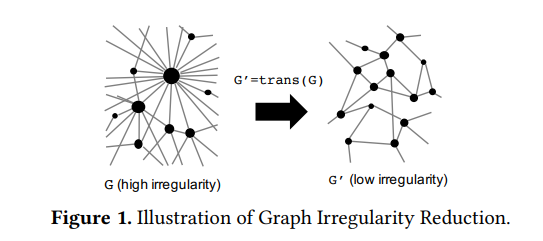
\includegraphics{C:/Users/workspace/cnn-compiler-notebook/figures/1568654140133.png}

  Details can be found at
  \href{https://github.com/OrdinaryCrazy/cnn-compiler-notebook/blob/master/Studying\%20Note/tigr.md}{Github
  link}
\item
  Fast train GNN on dense hardware

  Permute nodes to expose low bandwidth structure and express GNN
  propagation in terms of application of dense matrix multiply
  primitive.

  Details can be found at
  \href{https://github.com/OrdinaryCrazy/cnn-compiler-notebook/blob/master/paper-reading-note/fast-training\%20of\%20sparse\%20gnn\%20on\%20dense\%20hardware.pdf}{Github
  link}
\end{itemize}

\hypertarget{header-n1832}{%
\subsection{General Model Project: PyTorch
Geometric}\label{header-n1832}}

Github Project
\href{https://github.com/rusty1s/pytorch_geometric}{rusty1s/pytorch\_geometric}
implements many important GNN models with general GNN model Message
Passing Neural Network, and builds an end-to-end graph data loading to
testing model architecture. Detail studying note can be found at
\href{https://github.com/OrdinaryCrazy/cnn-compiler-notebook/blob/master/Studying\%20Note/learn-pytorch-geometric.md}{Github
Link}

\begin{figure}
\centering
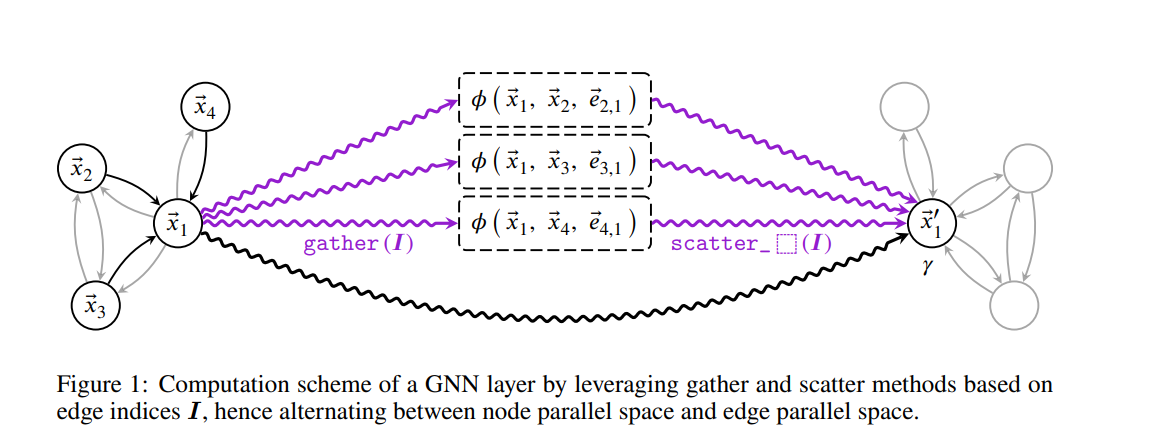
\includegraphics{C:/Users/workspace/cnn-compiler-notebook/figures/1568652726168.png}
\caption{}
\end{figure}

I modified this project for the following research: Code can be found at
\href{https://github.com/OrdinaryCrazy/cnn-compiler-notebook/tree/master/pytorch_geometric}{Github
Link}

\begin{itemize}
\item
  Profiling of GNN models

  Complexity analysis of MPNN network

  Details can be found at
  \href{https://github.com/OrdinaryCrazy/cnn-compiler-notebook/blob/master/weekly-report/weeklyreport0722-0728.pdf}{Github
  link}\\
  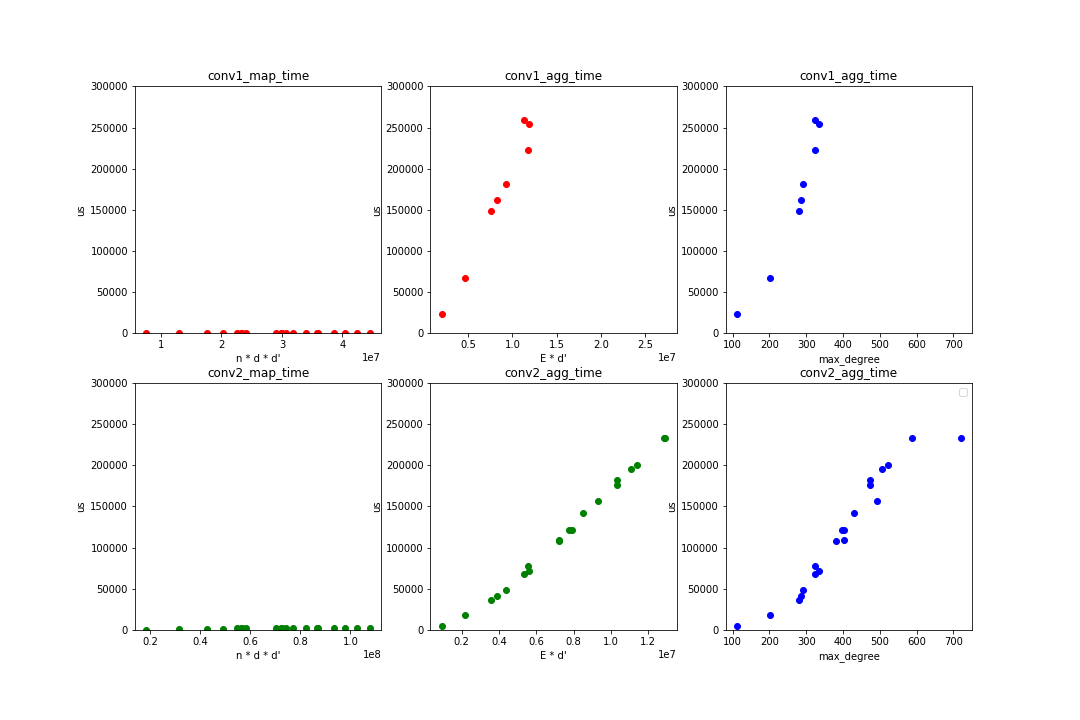
\includegraphics{C:/Users/workspace/cnn-compiler-notebook/figures/ppi_plot_cpu.png}
\item
  Visualization of Pooling effectiveness

  In topology domain: \textbf{Less nodes}

  \begin{figure}
  \centering
  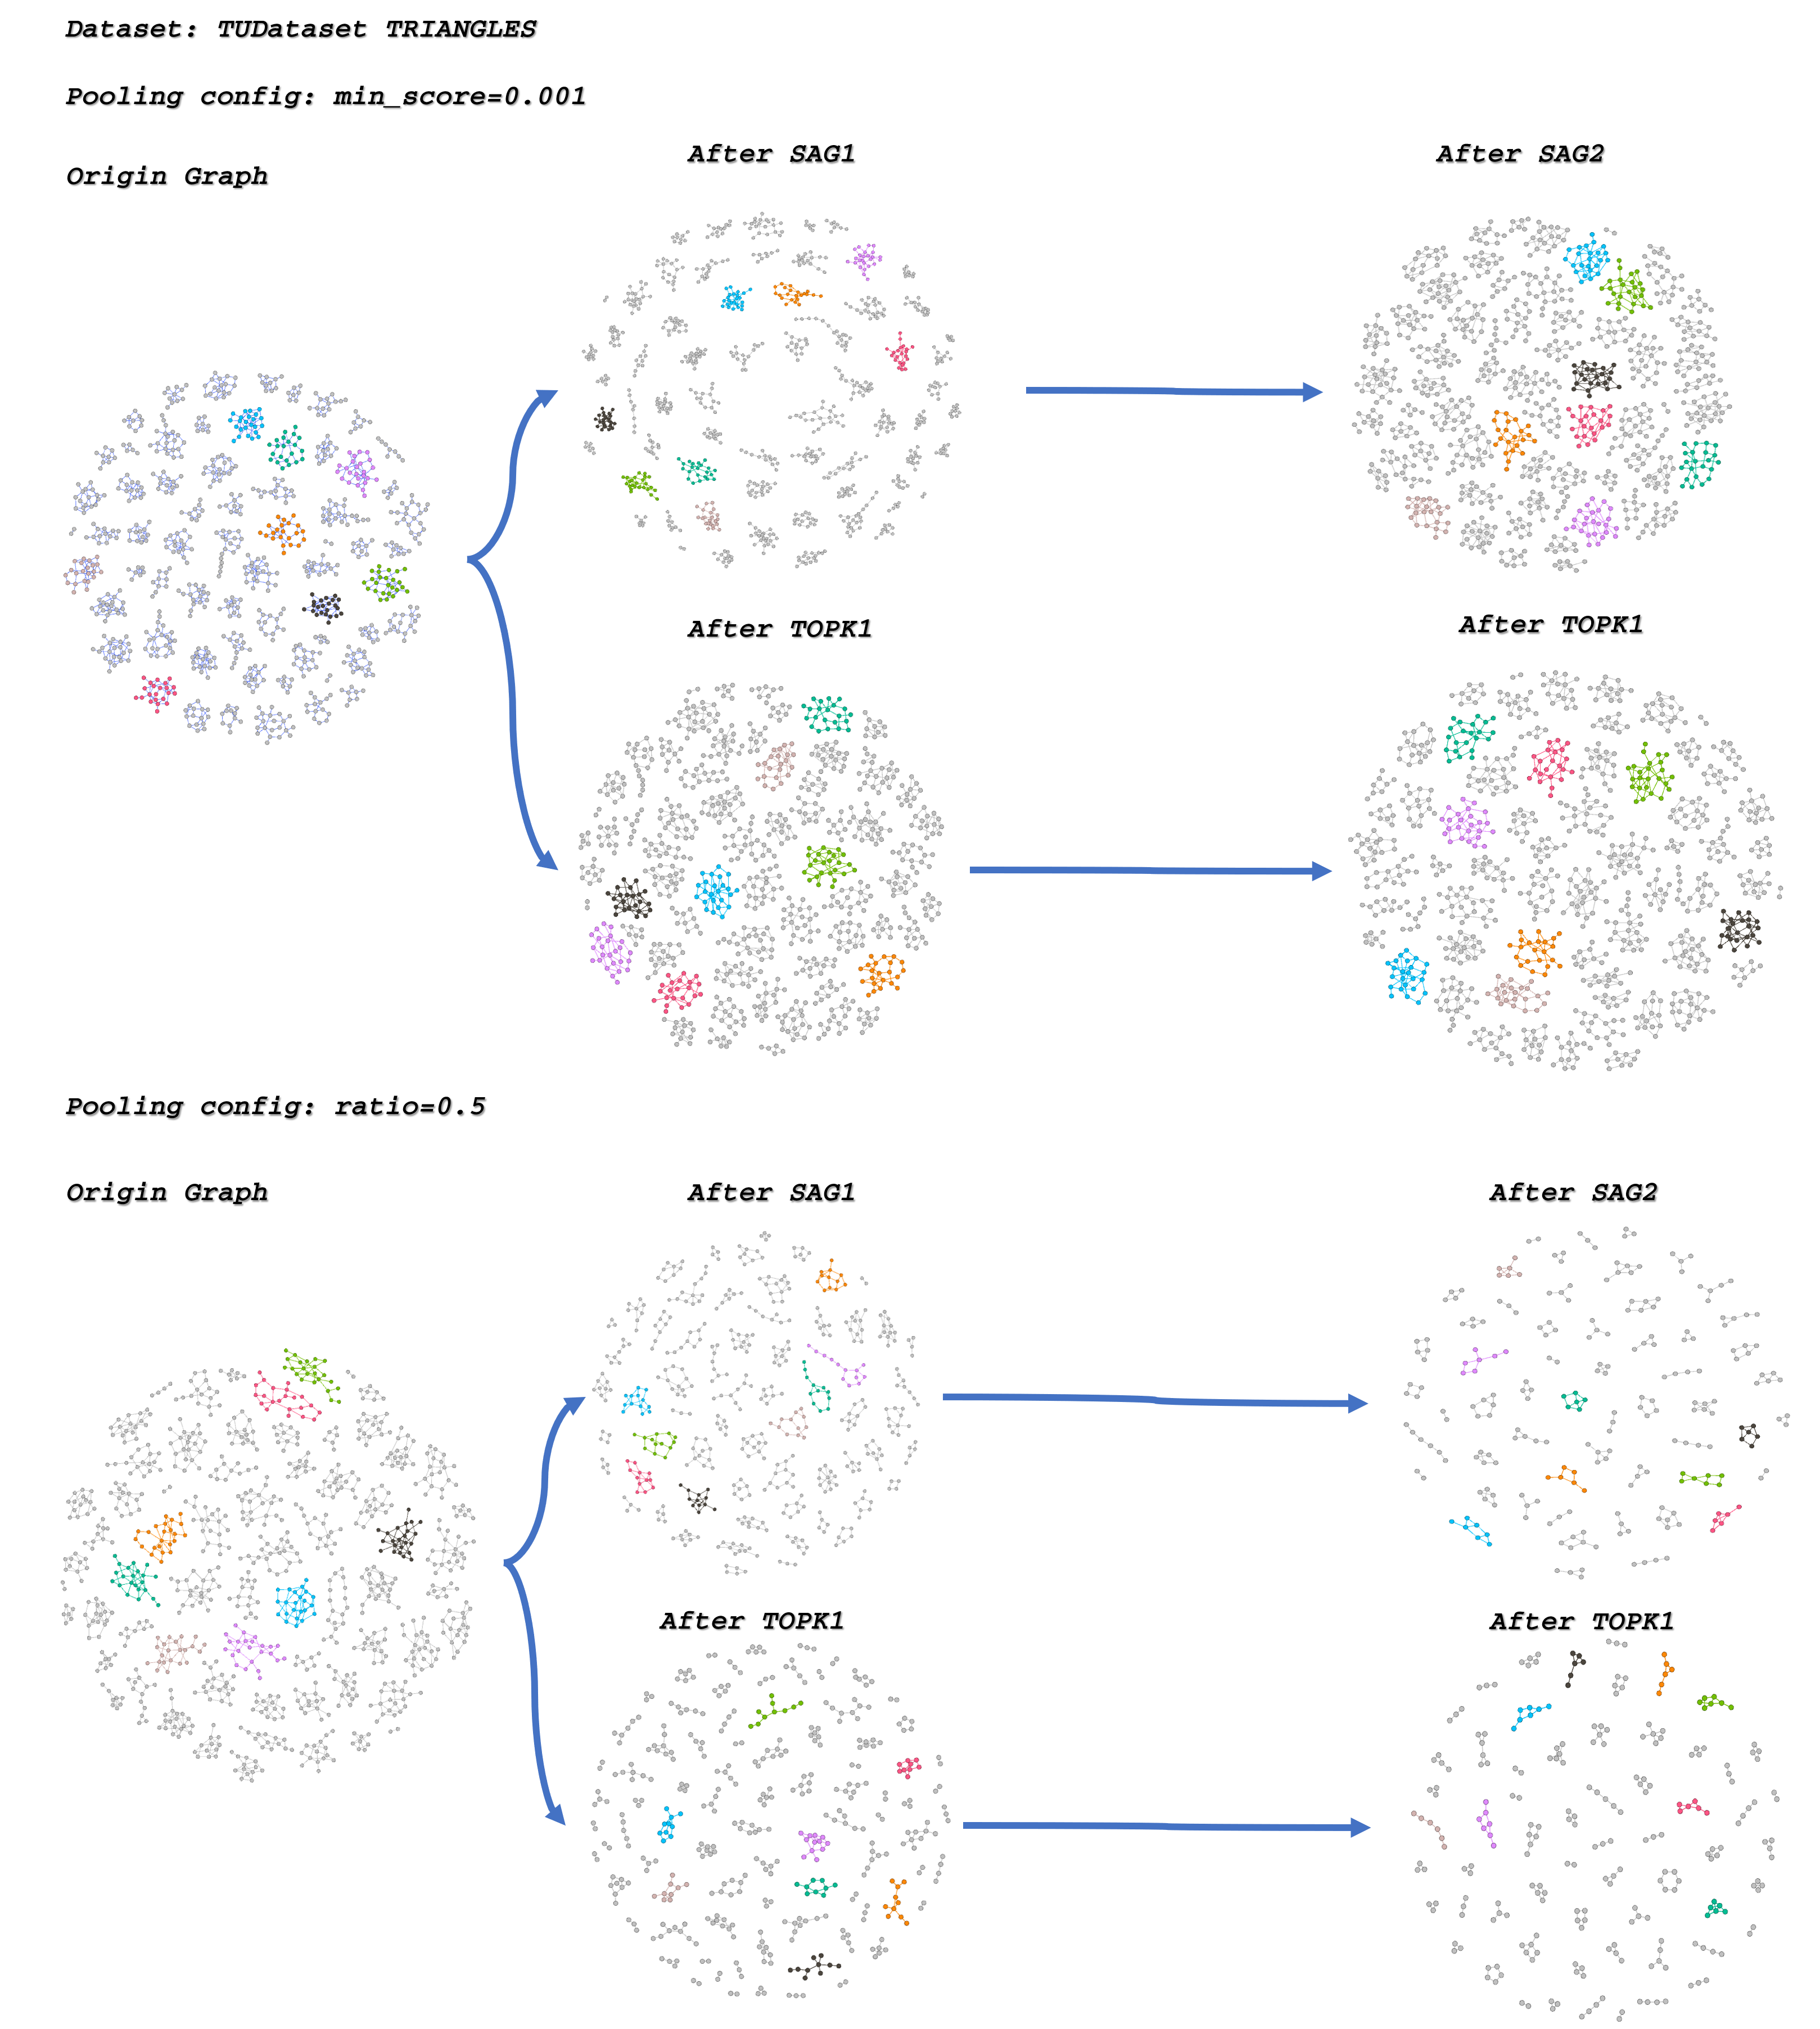
\includegraphics{C:/Users/workspace/cnn-compiler-notebook/figures/pool.png}
  \caption{}
  \end{figure}

  In embedding domain: \textbf{Maintenance of group structure and
  similarity}

  \begin{figure}
  \centering
  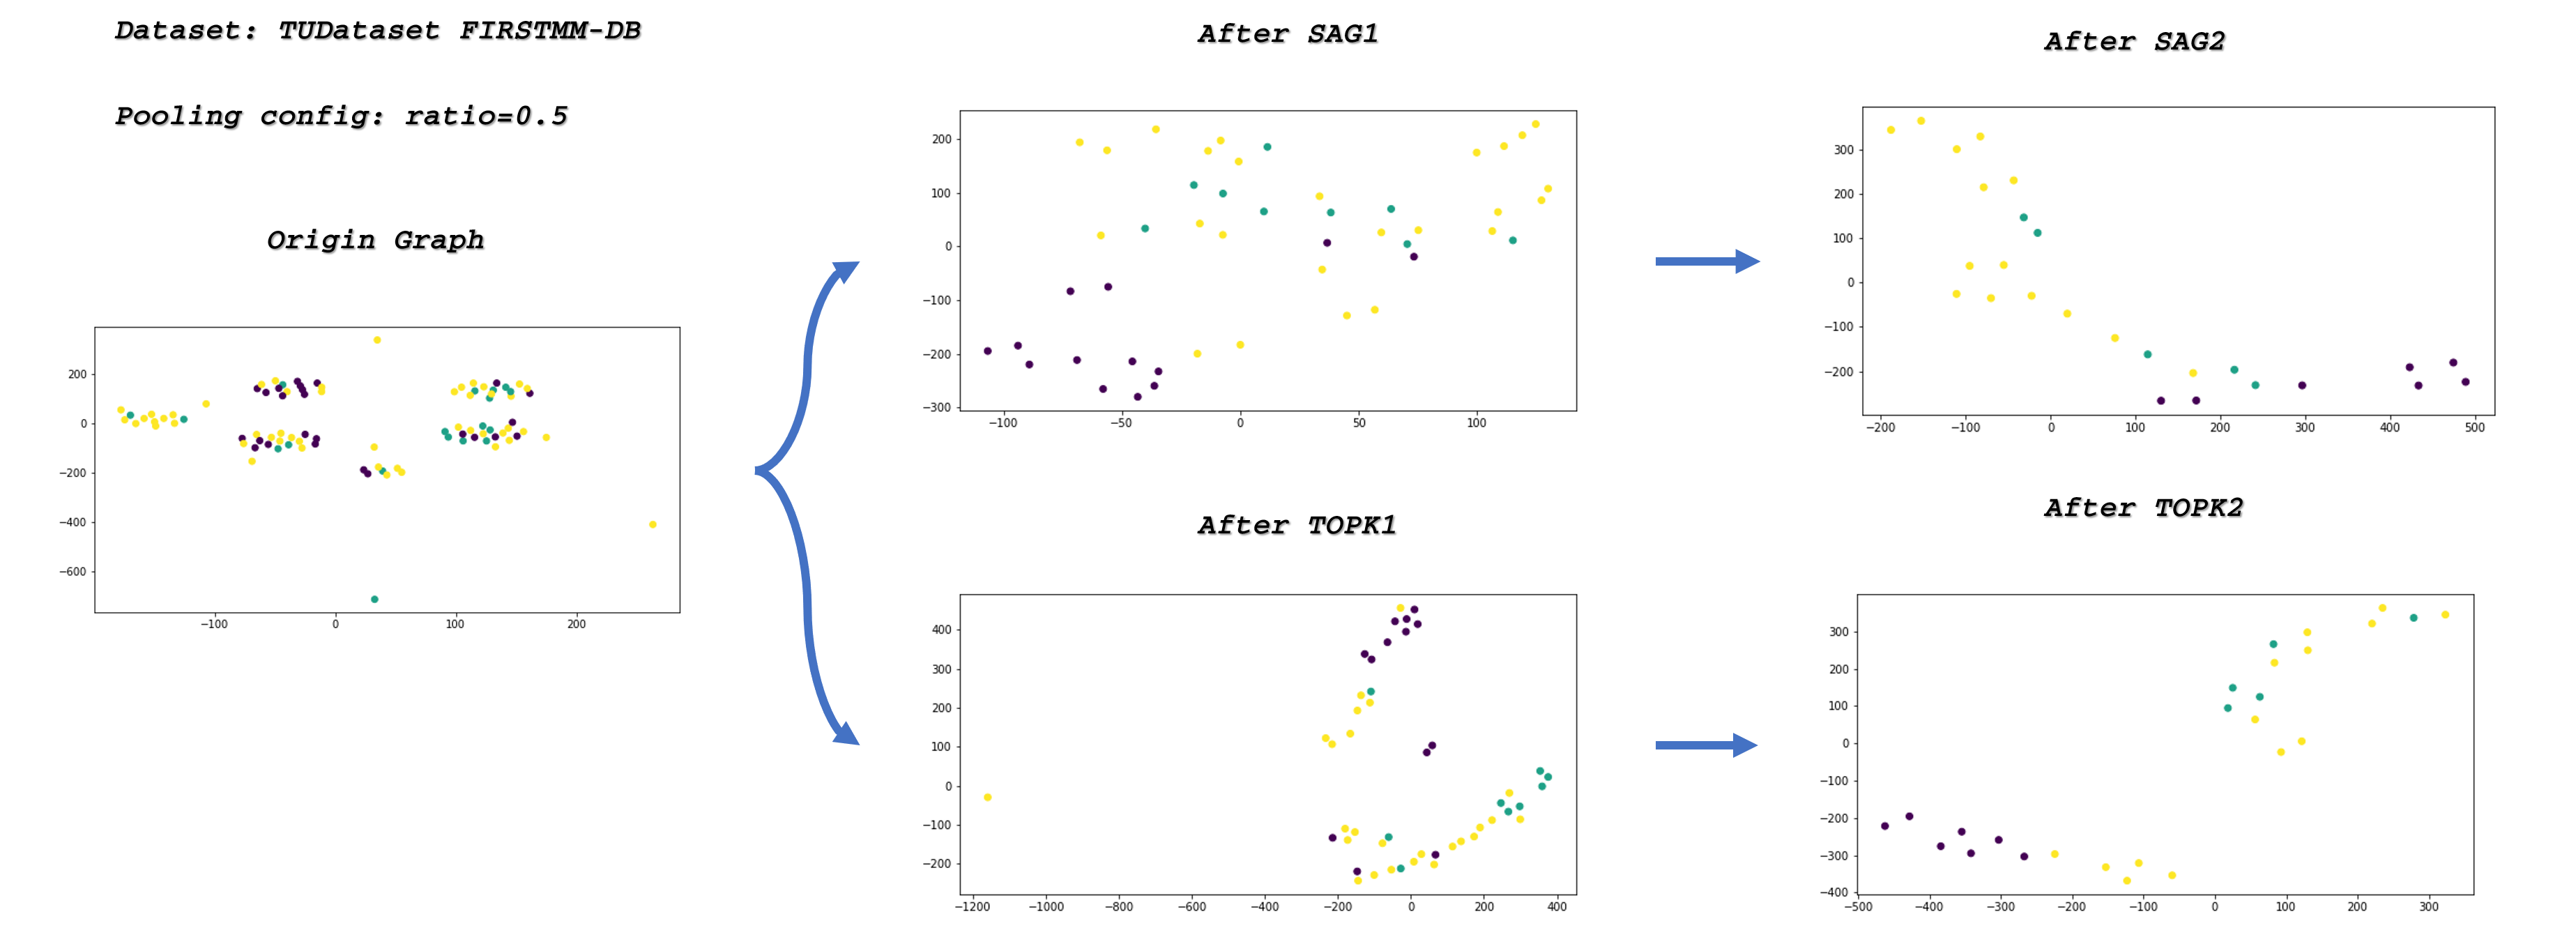
\includegraphics{C:/Users/workspace/cnn-compiler-notebook/figures/pool2.png}
  \caption{}
  \end{figure}

  Details can be found at
  \href{https://github.com/OrdinaryCrazy/cnn-compiler-notebook/blob/master/GNN-jupyter-code/topk-pooling\%20visualization.ipynb}{Github
  link}
\end{itemize}

\hypertarget{header-n1851}{%
\subsection{Hierarchically Aggregated computation Graphs
(HAGs)}\label{header-n1851}}

\hypertarget{header-n1852}{%
\subsubsection{Paper reading and Key idea}\label{header-n1852}}

Represent common neighbors across different nodes using aggregation
hierarchies, which eliminates redundant computation and unnecessary data
transfers in both GNN training and inference.

\begin{figure}
\centering
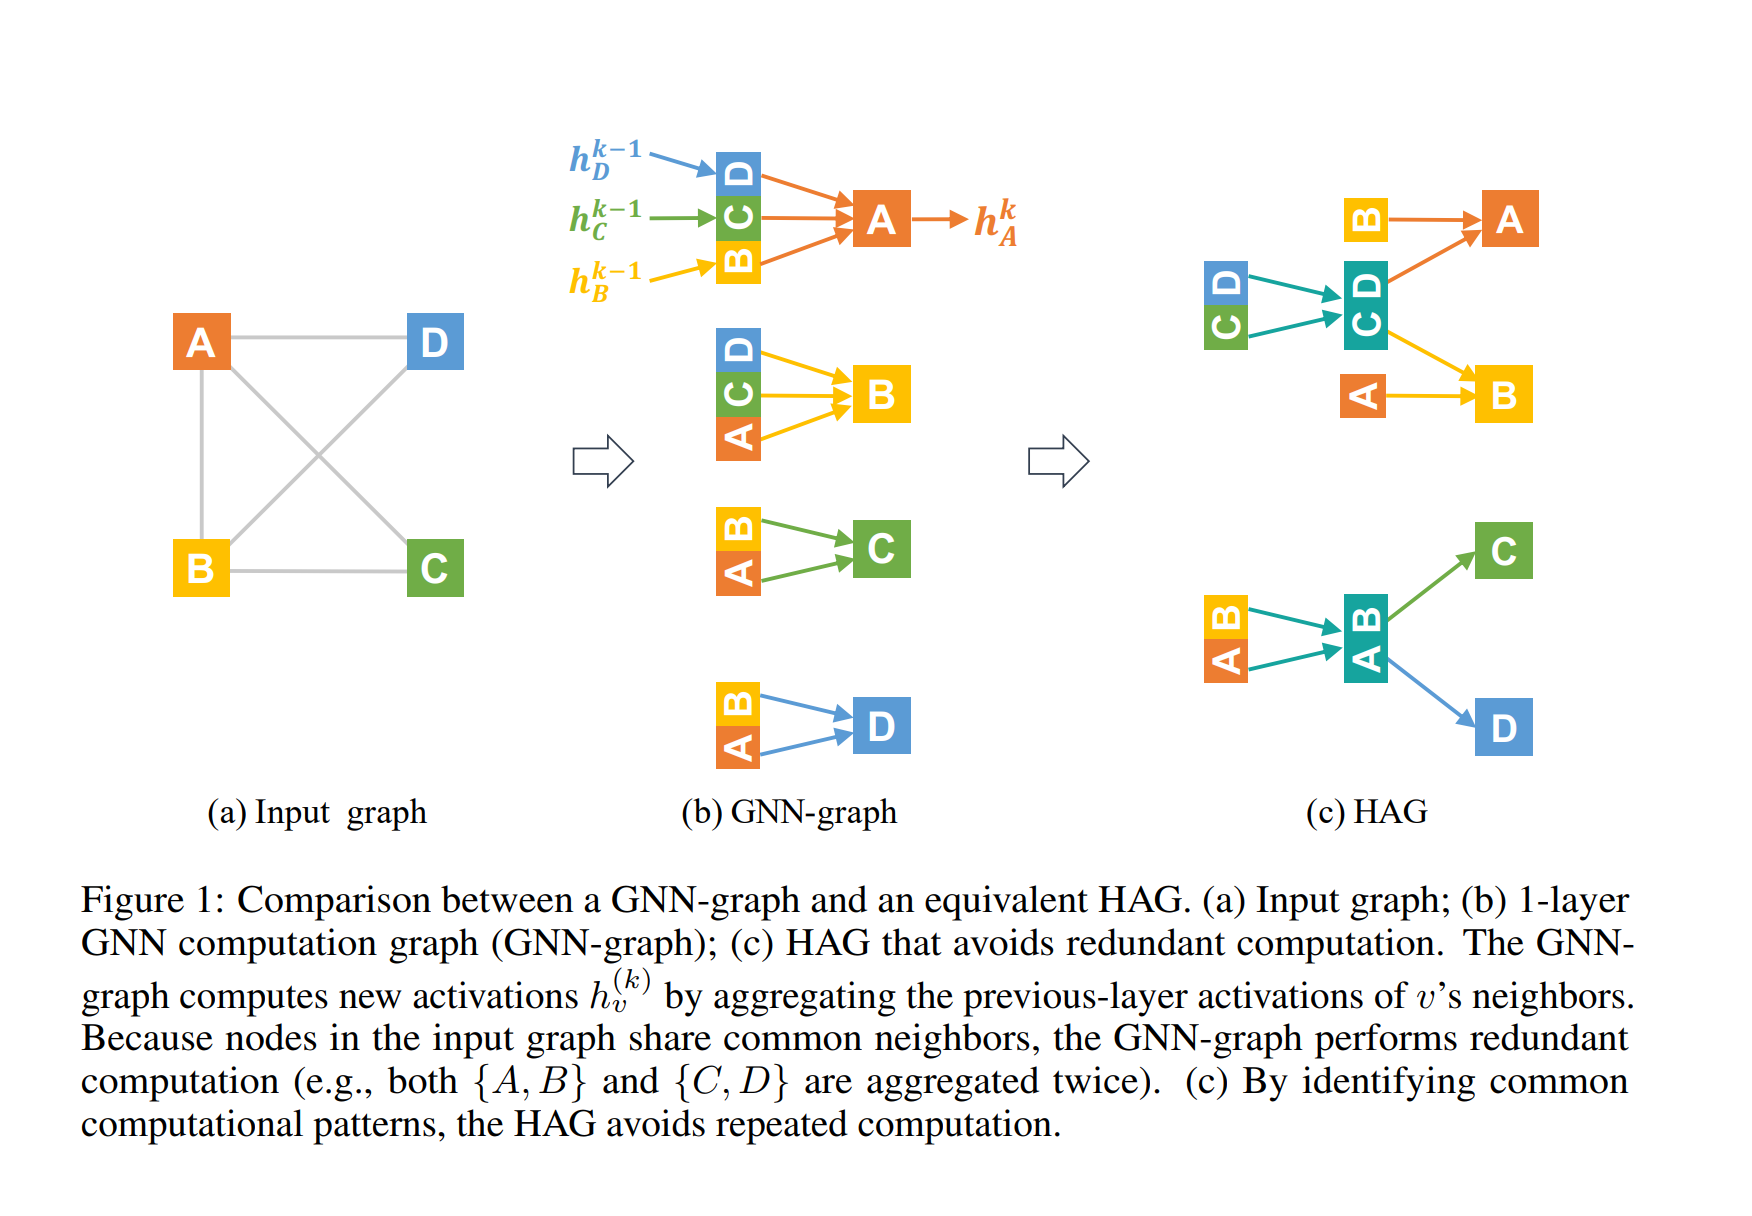
\includegraphics{C:/Users/workspace/cnn-compiler-notebook/figures/1568650351172.png}
\caption{}
\end{figure}

Problems:

\begin{itemize}
\item
  Maybe Not Optimal, But No Better Idea
\item
  Did not release code or details the heap maintenance method
\item
  More Discussion:

  \begin{enumerate}
  \def\labelenumi{\arabic{enumi}.}
  \item
    Understanding of the model:

    Details can be found at
    \href{https://github.com/OrdinaryCrazy/cnn-compiler-notebook/blob/master/weekly-report/weeklyreport0722-0728.pdf}{Github
    link}

    \begin{figure}
    \centering
    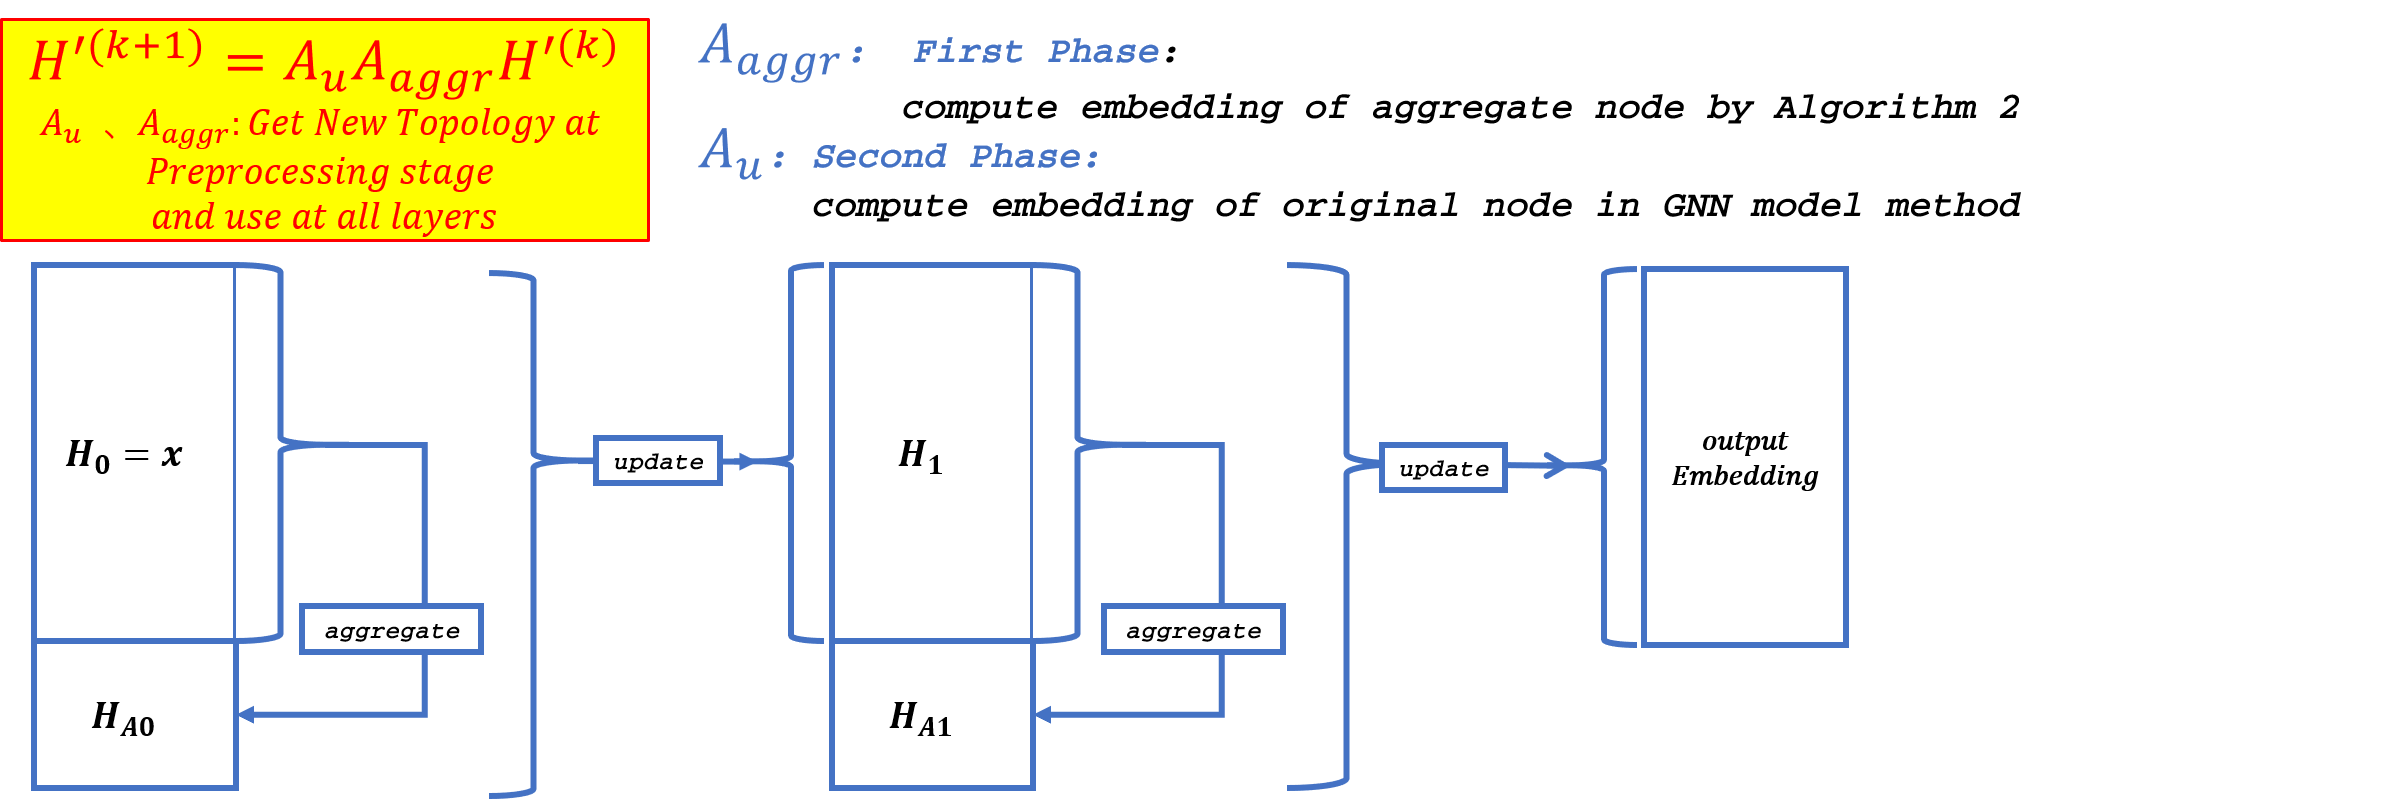
\includegraphics{C:/Users/workspace/cnn-compiler-notebook/figures/HAG.png}
    \caption{}
    \end{figure}
  \item
    Detailed description about max redundancy computation:

    Details can be found at
    \href{https://github.com/OrdinaryCrazy/cnn-compiler-notebook/blob/master/weekly-report/weeklyreport0729-0804.pdf}{Github
    link}
  \end{enumerate}

  \begin{figure}
  \centering
  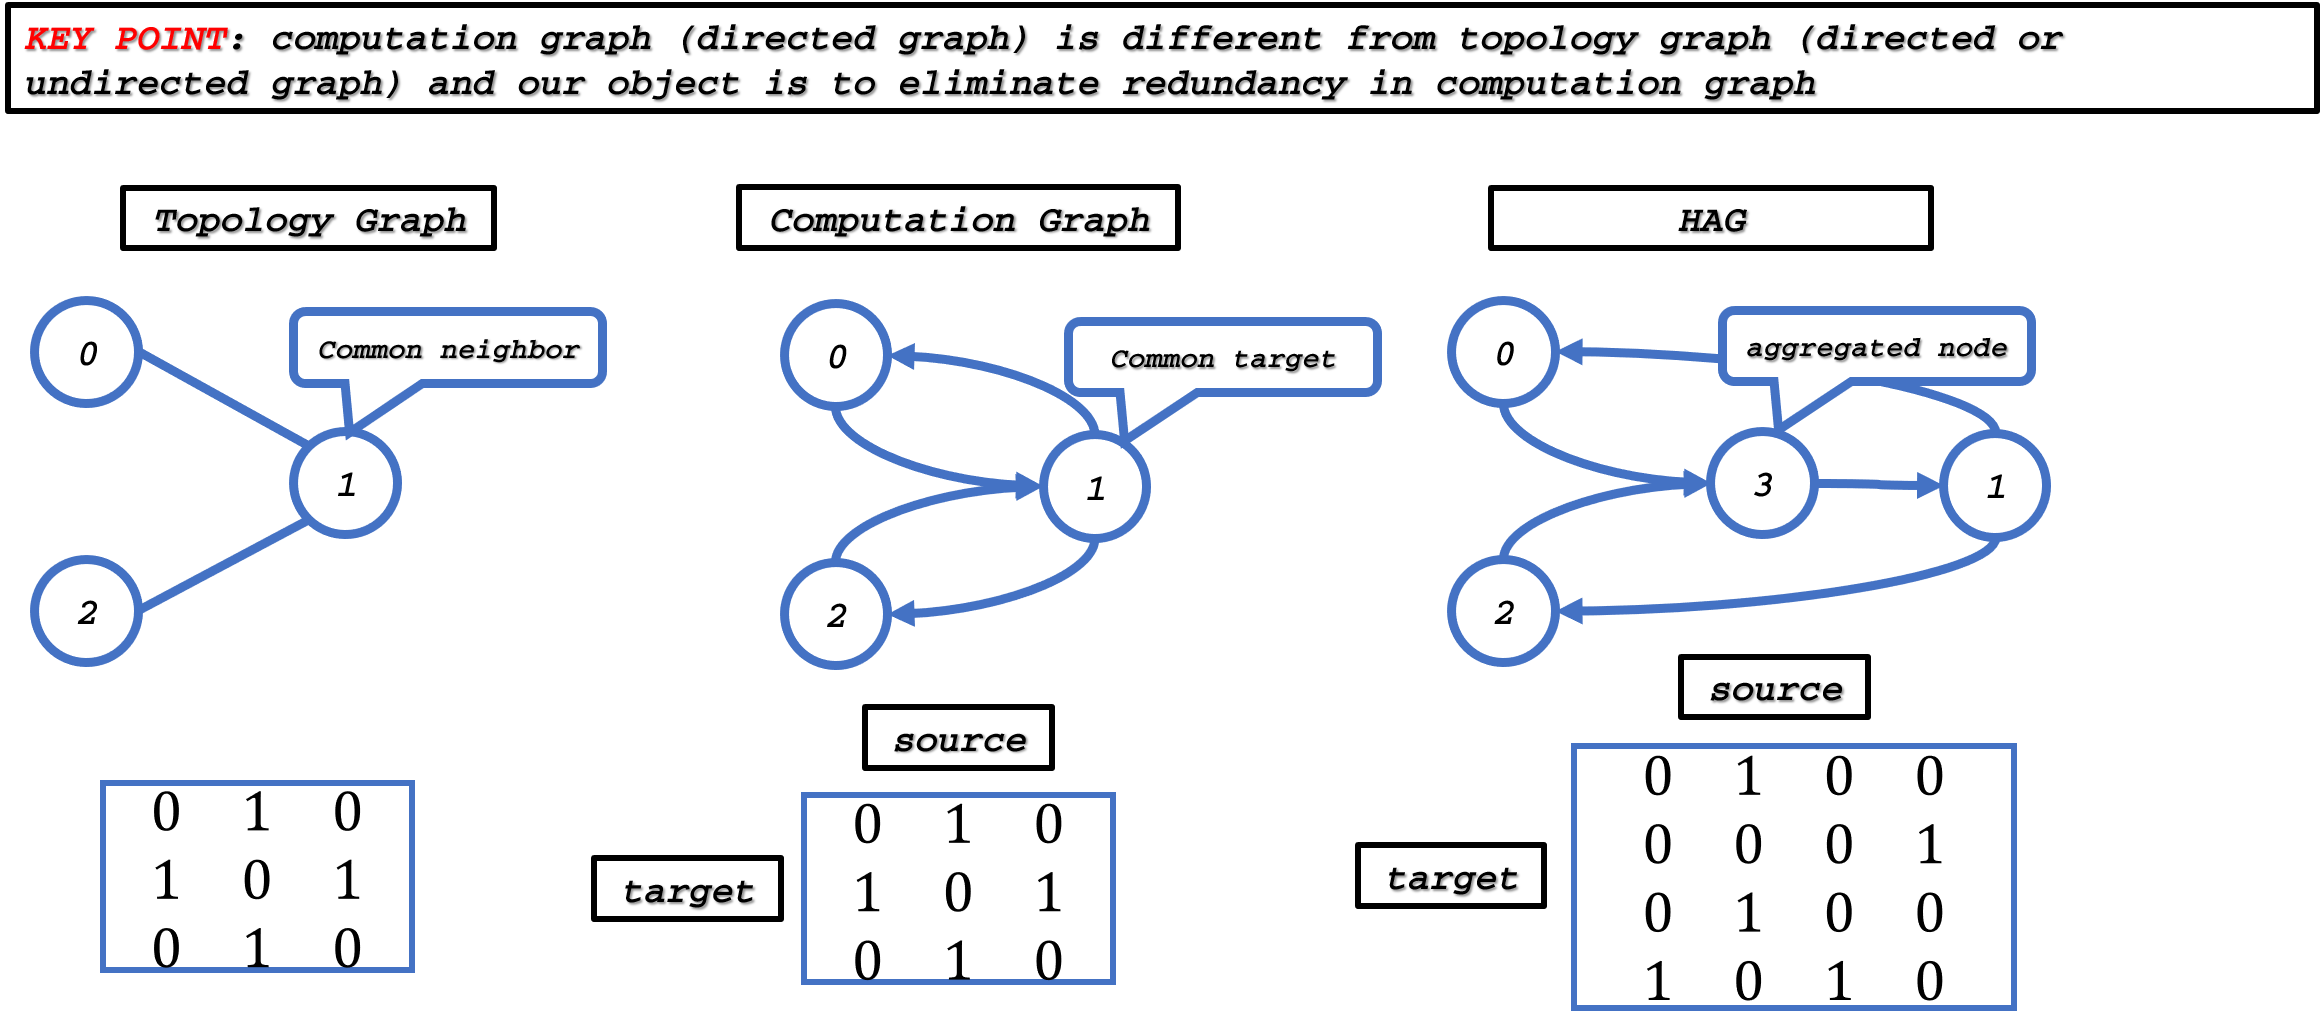
\includegraphics{C:/Users/workspace/cnn-compiler-notebook/figures/computation and topology.png}
  \caption{}
  \end{figure}
\end{itemize}

\hypertarget{header-n1870}{%
\subsubsection{Reimplementation}\label{header-n1870}}

Release
\href{https://github.com/OrdinaryCrazy/cnn-compiler-notebook/blob/master/GNN-jupyter-code/HAG.py}{HAG
model Version 0.0}

More details can be found at
\href{https://github.com/OrdinaryCrazy/cnn-compiler-notebook/blob/master/weekly-report/weeklyreport0729-0804.pdf}{Tutorial}
and
\href{https://github.com/OrdinaryCrazy/cnn-compiler-notebook/tree/master/HAG}{Github
build}

\hypertarget{header-n1873}{%
\section{Motion-Vector based video Object
Detection}\label{header-n1873}}

\hypertarget{header-n1874}{%
\subsection{Tasks}\label{header-n1874}}

\hypertarget{header-n1875}{%
\subsubsection{Proof of mathmatical principal of
DFF}\label{header-n1875}}

We try to proof the existence of a linear transformation that maps the
feature map of key frame to the feature map of non-key frames based on
the motion information:

\begin{quote}
Given a convolution operation \(\mathbb{C}\), \(\forall\) frame
\(\mathcal{A}\) and \(\mathcal{B}\), as well as the corresponding
feature maps \(\mathcal{A'}\) and \(\mathcal{B'}\), \(\exists\) a linear
transformation
\(\mathcal{T} = \mathcal{C}^{-1}\cdot \mathcal{M}_{\mathcal{A} \to \mathcal{B}} \cdot \mathcal{C}\),
such that
\(\mathcal{B'} = \mathcal{A'} \cdot \mathcal{T} + \mathcal{\delta'}\),
where \(\mathcal{\delta'} = \mathcal{\delta}C\), where
\(\mathcal{M}_{\mathcal{A} \to \mathcal{B}}\) and \(\mathcal{\delta}\)
are motion and error information extracted from motion vector and
residual map respectively.
\end{quote}

And the error term of residual map will not explode after a sequence of
convolution operations:

\begin{quote}
Given a convolution operation \(\mathbb{C}\) with unit normality and an
error information \(\delta \sim \mathcal{N}(0, \sigma^2)\), the error
information \(\delta'\) after convolution operation enjoys
convolution-invariance, \emph{i.e.},
\(\delta' = \delta C \sim \mathcal{N}(0, \sigma^2)\).
\end{quote}

Details can be found at
\href{https://github.com/OrdinaryCrazy/cnn-compiler-notebook/blob/master/weekly-report/Rivulet_Proof.pdf}{Github
link}

\hypertarget{header-n1883}{%
\subsubsection{Motion Vector Feature Flow Version3}\label{header-n1883}}

\hypertarget{header-n1884}{%
\paragraph{Idea}\label{header-n1884}}

Rather than just scale the motion vector by 1x1 Convolutional Layer, we
try to build a more complicated MV\_Net try to improve the quality
of motion vector used at feature map level. MV\_Net is piced as
following:
\newpage
\begin{figure}
\centering
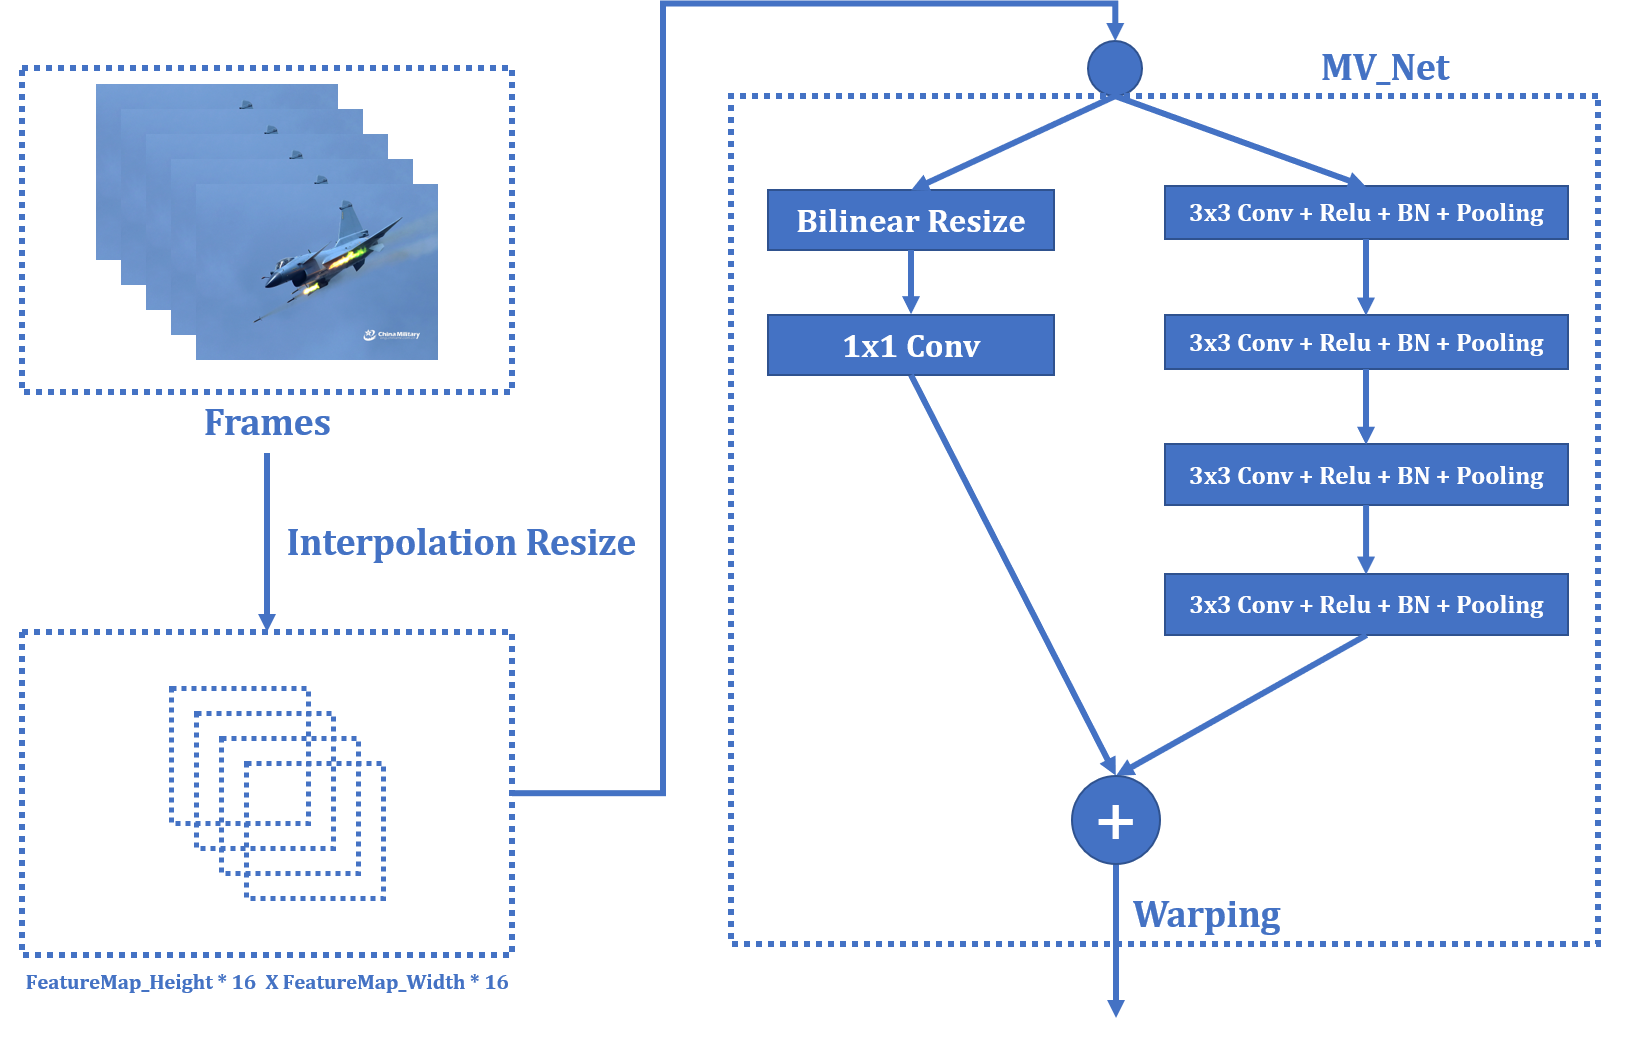
\includegraphics{C:/Users/workspace/cnn-compiler-notebook/figures/mvnet.png}
\caption{}
\end{figure}

\hypertarget{header-n1887}{%
\paragraph{Result and Discussion}\label{header-n1887}}

We get MAP@5 = 0.6225 with above MV\_Net architecture, some points we
discussed in the design:

\begin{itemize}
\item
  MVFF-Object-Detection task is sensitive to the information loss in
  integer-times scale and width-height-same-ratio scale of movtion
  vector in pooling process, so we need firstly use interpolation
  (non-integer-times) scale to scale the movtion vector to a
  integer-times of\\
  feature map shape (16*feat-map-width, 16*feat-map-height)

  Details can be found at
  \href{https://github.com/OrdinaryCrazy/cnn-compiler-notebook/blob/master/weekly-report/weeklyreport0819-0825.pdf}{Github
  link}
\end{itemize}

Code find at
\href{https://github.com/OrdinaryCrazy/mvff-sideversions}{MVFF-Version3}

File organization same as
\href{https://github.com/msracver/Deep-Feature-Flow}{Deep Feature Flow
for Video Recognition}

\hypertarget{header-n1895}{%
\subsubsection{Motion Vector Feature Flow Version4}\label{header-n1895}}

\hypertarget{header-n1896}{%
\paragraph{Idea}\label{header-n1896}}

Use DMC-Net like structure to fine-tune the motion vector, try to gain
more motion information form residual data under optical flow guidence.

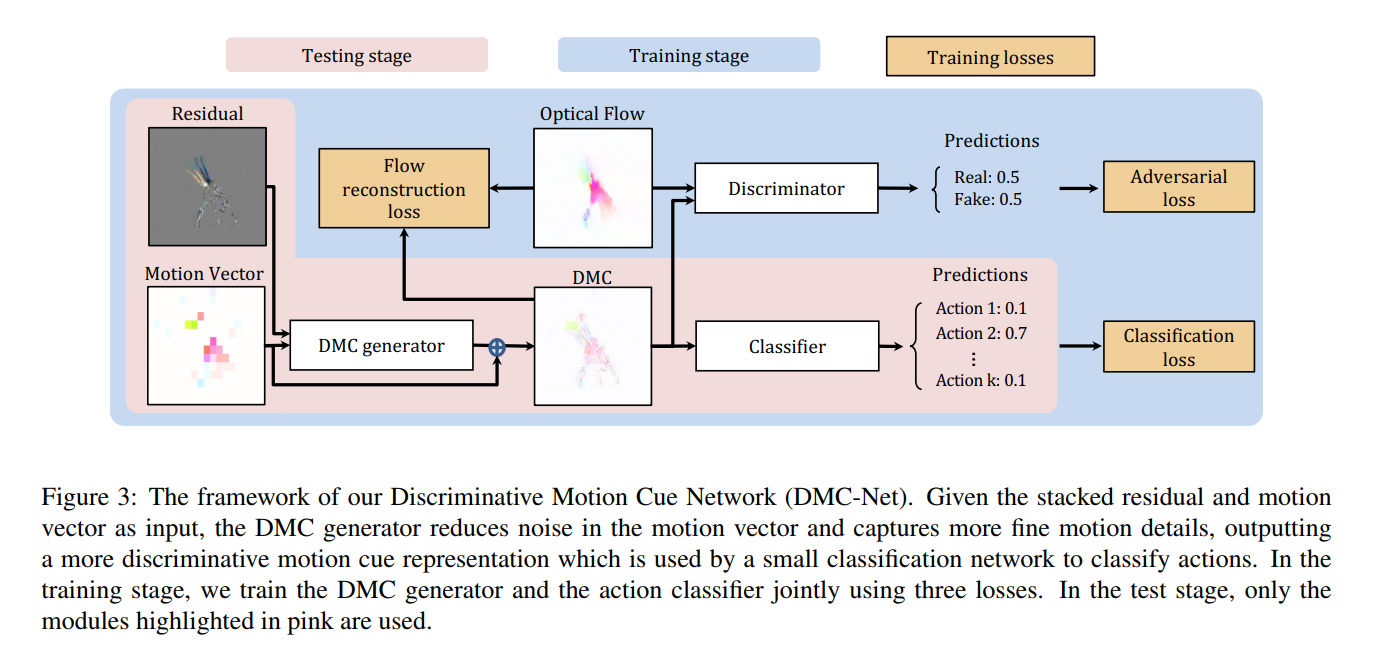
\includegraphics{C:/Users/workspace/cnn-compiler-notebook/figures/1566861769179.png}\\
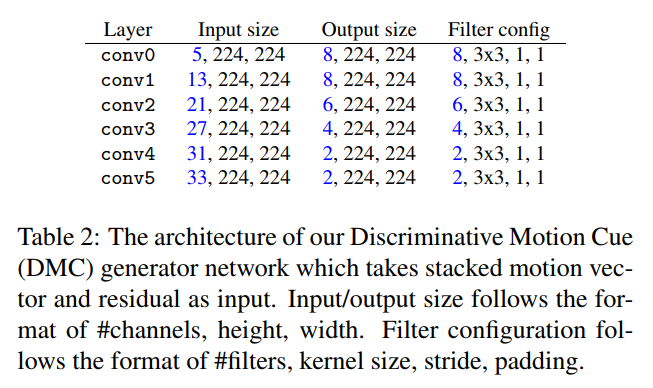
\includegraphics{C:/Users/workspace/cnn-compiler-notebook/figures/1566862456389.png}

DMC-Net details can be found at
\href{\%5Bhttps://github.com/OrdinaryCrazy/cnn-compiler-notebook/blob/master/Studying\%20Note/DMC-Net.md\%5D(https://github.com/OrdinaryCrazy/cnn-compiler-notebook/blob/master/Studying\%20Note/DMC-Net.md)}{Github
Link}

\hypertarget{header-n1900}{%
\paragraph{Result and Discussion}\label{header-n1900}}

Result of MVFF-Version4-without optical flow guidence: MAP@5 = 0.5091.

Maybe we need extract optical flow from the dataset first.

Code find at
\href{https://github.com/OrdinaryCrazy/mvff-sideversions/tree/master/Version4}{MVFF-Version4}

\hypertarget{header-n1904}{%
\subsubsection{Motion Vector Output Flow Step-Performance
Curve}\label{header-n1904}}

We tried different steps of MVOF to approximate the result of DFF and
accelerate it, trying to analyse motion vector propagation at output
level.

\begin{figure}
\centering
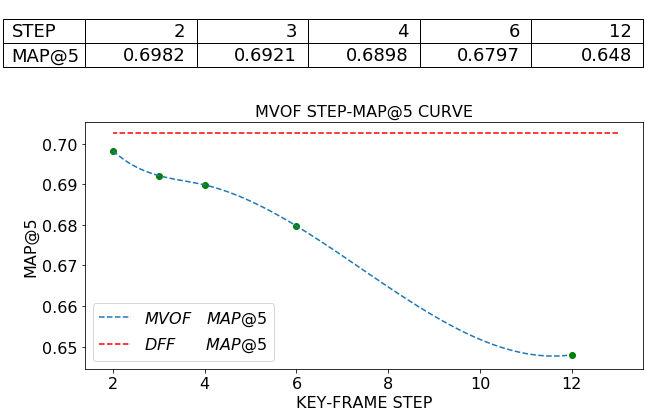
\includegraphics{C:/Users/workspace/cnn-compiler-notebook/figures/mvof.png}
\caption{}
\end{figure}

\hypertarget{header-n1907}{%
\section{Quantum Computing Learning}\label{header-n1907}}

\hypertarget{header-n1908}{%
\subsection{First stage: From bits to qubits: Basical Concepts and
Algorithm of Quantum Computing}\label{header-n1908}}

\hypertarget{header-n1909}{%
\subsubsection{What Is a QPU? }\label{header-n1909}}

\begin{itemize}
\item
  QPU (Quantum Processing Unit) is a co-processor 
\item
  QPU has ability to dramatically extend the kinds of problems that are
  tractable within computing. 
\item
  The CPU issues the QPU co-processor commands only to initiate tasks
  suited to its capabilities.
\end{itemize}

\hypertarget{header-n1917}{%
\subsubsection{Native QPU Instructions }\label{header-n1917}}

\begin{itemize}
\item
  Conventional high-level languages are commonly used to control
  lower-level QPU instructions. 
\item
  Essential QPU instruction set 
\end{itemize}

\hypertarget{header-n1923}{%
\subsubsection{Simulator Limitations }\label{header-n1923}}

\begin{itemize}
\item
  One measure of the power of a QPU is the number of qubits it has
  available to operate on. 
\item
  Each qubit added to simulation will double the memory required to run
  the simulation, cutting its speed in half.
\end{itemize}

\hypertarget{header-n1929}{%
\subsubsection{QPU Versus GPU: }\label{header-n1929}}

Some Common Characteristics What it's like to program a QPU:

\begin{itemize}
\item
  It is very rare that a program will run entirely on a QPU. Usually, a
  program runnning on a CPU will issue QPU instructions, and later
  retrieve the results.
\item
  Some tasks are very suited to the QPU, and others are not.
\item
  The QPU runs on a separate clock from the CPU, and usually has its own
  dedicated hardware interfaces to external devices (such as optical
  outputs).
\item
  A typical QPU has its own special RAM, which the CPU cannot
  efficiently access.
\item
  A simple QPU will be one chip accessed by a laptop, or even perhaps
  eventually an area within another chip. A more advanced QPU is a large
  and expensive addon, and always requires special cooling.
\item
  When a computation is done, a projection of the result is returned to
  the CPU, and most of the QPU's internal working data is discarded.
\item
  QPU debugging can be very tricky, requiring special tools and
  techniques, Stepping through a program can be difficult, and often the
  best approcah is to make changes to the program and observe their
  effect on the output.
\item
  Optimizations that speed up one QPU may slow down another.
\end{itemize}

\hypertarget{header-n1948}{%
\subsection{\texorpdfstring{\sout{Second stage: Great idea evolution and
Important
Works}}{Second stage: Great idea evolution and Important Works}}\label{header-n1948}}

\hypertarget{header-n1949}{%
\subsection{\texorpdfstring{\sout{Third stage: On-going Front Problem
and
Research}}{Third stage: On-going Front Problem and Research}}\label{header-n1949}}

\hypertarget{header-n1950}{%
\subsection{\texorpdfstring{\sout{Fourth stage: Research
directions}}{Fourth stage: Research directions}}\label{header-n1950}}

\end{document}
